% sou_workforce_pell.tex -- Deck B.
%
% Audience: SOU officials, community members, with secondary asks
% addressed to HECC and the Oregon Workforce & Talent Development
% Board (WTDB).
%
% Framing: SOU revenue diversification through a new federal
% category -- Workforce Pell -- created by the May 18, 2026 final
% rule and effective July 20, 2026.  Most of the audience has not
% heard of Workforce Pell.  The deck explains it, argues that
% universities are uniquely positioned to deliver it, shows that
% the Rogue Valley has the demand to support it, and asks SOU
% leadership to include a Workforce Pell track in the
% revenue-diversification proposal currently being drafted.
%
% Visual language: dark tensor-fusion (matches Deck A south_fusion).
% Libertinus type, cream-on-deep-navy palette, isometric cube,
% schematic vector geometry.
%
% Build (xelatex required for fontspec / Libertinus OTF):
%   cd decks
%   latexmk -xelatex sou_workforce_pell.tex
%
\PassOptionsToPackage{table,xcdraw}{xcolor}
\documentclass[aspectratio=169,11pt]{beamer}

\usepackage{fontspec}
\usepackage{booktabs}
\usepackage{array}
\usepackage{tikz}
\usetikzlibrary{positioning,arrows.meta,fit,backgrounds,calc,shapes.geometric,decorations.pathreplacing,decorations.markings}

\providecommand{\fact}[1]{}
\renewcommand{\fact}[1]{\csname fact@#1\endcsname}
\InputIfFileExists{facts.tex}{}{}

%-----------------------------------------------------------------------
% Fonts -- Libertinus family.
%-----------------------------------------------------------------------
\setmainfont{LibertinusSerif}[
  Extension      = .otf,
  UprightFont    = *-Regular,
  ItalicFont     = *-Italic,
  BoldFont       = *-Bold,
  BoldItalicFont = *-BoldItalic,
  Ligatures      = TeX,
]
\setsansfont{LibertinusSans}[
  Extension      = .otf,
  UprightFont    = *-Regular,
  ItalicFont     = *-Italic,
  BoldFont       = *-Bold,
  Ligatures      = TeX,
  Scale          = 0.94,
]
\setmonofont{LibertinusMono}[
  Extension      = .otf,
  UprightFont    = *-Regular,
  Scale          = 0.88,
  Ligatures      = TeX,
]
\newfontfamily{\displayfont}{LibertinusSerifDisplay}[
  Extension      = .otf,
  UprightFont    = *-Regular,
  Ligatures      = TeX,
]

%-----------------------------------------------------------------------
% Theme.
%-----------------------------------------------------------------------
\newif\ifLightMode \LightModefalse
\InputIfFileExists{_deck_theme.tex}{}{}

%-----------------------------------------------------------------------
% Palette.
%-----------------------------------------------------------------------
\ifLightMode
  \definecolor{bgDeep}{HTML}{EFE7D2}
  \definecolor{bgBase}{HTML}{FAF6EC}
  \definecolor{bgRaised}{HTML}{F0E9D8}
  \definecolor{bgCard}{HTML}{EDE5D0}
  \definecolor{textPrimary}{HTML}{1A1A1A}
  \definecolor{textSecondary}{HTML}{3A3A3A}
  \definecolor{textMuted}{HTML}{6A6A6A}
  \definecolor{textDim}{HTML}{9A9A9A}
  \definecolor{lineSoft}{HTML}{D5CFC0}
  \definecolor{lineMid}{HTML}{A8A293}
  \definecolor{lineStrong}{HTML}{7A746A}
  \definecolor{oil}{HTML}{B86F30}
  \definecolor{oilBright}{HTML}{D99A5F}
  \definecolor{oilDeep}{HTML}{7A4A1F}
  \definecolor{feedback}{HTML}{2F7A73}
  \definecolor{cSou}{HTML}{B0142A}
  \definecolor{cSoredi}{HTML}{2F7A73}
  \definecolor{cBiz}{HTML}{8C4F1E}
  \definecolor{cRwp}{HTML}{6A4F9C}
  \definecolor{cWr}{HTML}{B5803C}
  \definecolor{cPell}{HTML}{1F5A8C}
\else
  \definecolor{bgDeep}{HTML}{070A0F}
  \definecolor{bgBase}{HTML}{0B0F17}
  \definecolor{bgRaised}{HTML}{131A23}
  \definecolor{bgCard}{HTML}{1A2230}
  \definecolor{textPrimary}{HTML}{E8E2D4}
  \definecolor{textSecondary}{HTML}{B6B2A6}
  \definecolor{textMuted}{HTML}{7D8493}
  \definecolor{textDim}{HTML}{4D5363}
  \definecolor{lineSoft}{HTML}{1F2630}
  \definecolor{lineMid}{HTML}{3A4250}
  \definecolor{lineStrong}{HTML}{5A6273}
  \definecolor{oil}{HTML}{D99A5F}
  \definecolor{oilBright}{HTML}{F4C08A}
  \definecolor{oilDeep}{HTML}{B86F30}
  \definecolor{feedback}{HTML}{5EB3A8}
  \definecolor{cSou}{HTML}{C8102E}
  \definecolor{cSoredi}{HTML}{5EB3A8}
  \definecolor{cBiz}{HTML}{D99A5F}
  \definecolor{cRwp}{HTML}{9B7FBF}
  \definecolor{cWr}{HTML}{F4C08A}
  \definecolor{cPell}{HTML}{6FA8DC}
\fi

%-----------------------------------------------------------------------
% Beamer chrome.
%-----------------------------------------------------------------------
\usetheme{default}
\setbeamertemplate{navigation symbols}{}
\setbeamercolor{background canvas}{bg=bgBase}
\setbeamercolor{normal text}{fg=textPrimary,bg=bgBase}
\setbeamercolor{frametitle}{fg=textPrimary,bg=bgBase}
\setbeamercolor{title}{fg=textPrimary}
\setbeamercolor{author}{fg=textMuted}
\setbeamercolor{date}{fg=textMuted}
\setbeamercolor{institute}{fg=textMuted}
\setbeamercolor{itemize item}{fg=oil}
\setbeamercolor{itemize subitem}{fg=textMuted}
\setbeamerfont{frametitle}{family=\rmfamily,series=\mdseries,size=\Large}
\setbeamertemplate{itemize item}{\color{oil}\rule[0.4ex]{0.6em}{0.5pt}}
\setbeamertemplate{itemize subitem}{\color{textMuted}\rule[0.4ex]{0.4em}{0.3pt}}

\newcommand{\eyebrow}[1]{%
  {\sffamily\fontsize{7.5pt}{9pt}\selectfont
   \color{textMuted}%
   \MakeUppercase{#1}%
  }%
}
\newcommand{\monoLabel}[1]{%
  {\ttfamily\fontsize{7.5pt}{9pt}\selectfont\color{textMuted}#1}%
}

\newcommand{\theEyebrowText}{}
\newcommand{\frametitleEyebrow}[1]{\renewcommand{\theEyebrowText}{#1}}
\setbeamertemplate{frametitle}{%
  \vskip 0.30cm
  \hspace*{1.0cm}%
  \begin{minipage}{\dimexpr\paperwidth-2.0cm\relax}%
    \eyebrow{\theEyebrowText}\par\vspace{2pt}%
    {\color{textPrimary}\rmfamily\fontsize{18pt}{21pt}\selectfont
     \insertframetitle\par}%
    \vspace{4pt}%
    {\color{lineMid}\rule{3.6em}{0.5pt}}%
    \hspace{2pt}%
    {\color{oil}\rule{1em}{0.5pt}}%
  \end{minipage}%
  \par\vspace{0.18cm}%
}

\setbeamertemplate{footline}{%
  \leavevmode
  \hbox{%
    \begin{beamercolorbox}[wd=\paperwidth,ht=2.4ex,dp=1.2ex,leftskip=1.0cm,rightskip=1.0cm]{}%
      \monoLabel{sou / workforce pell at sou}%
      \hfill
      \monoLabel{\insertframenumber\,/\,\inserttotalframenumber}%
    \end{beamercolorbox}%
  }%
}

%-----------------------------------------------------------------------
% Background -- hairline corner ticks.
%-----------------------------------------------------------------------
\setbeamertemplate{background}{%
  \begin{tikzpicture}[remember picture, overlay]
    \fill[bgBase] (current page.south west) rectangle (current page.north east);
    \draw[lineMid,line width=0.4pt]
      ([xshift=0.6cm,yshift=0.6cm]current page.south west) -- ++(0.25cm,0);
    \draw[lineMid,line width=0.4pt]
      ([xshift=0.6cm,yshift=0.6cm]current page.south west) -- ++(0,0.25cm);
    \draw[lineMid,line width=0.4pt]
      ([xshift=-0.6cm,yshift=0.6cm]current page.south east) -- ++(-0.25cm,0);
    \draw[lineMid,line width=0.4pt]
      ([xshift=-0.6cm,yshift=0.6cm]current page.south east) -- ++(0,0.25cm);
    \draw[lineMid,line width=0.4pt]
      ([xshift=0.6cm,yshift=-0.6cm]current page.north west) -- ++(0.25cm,0);
    \draw[lineMid,line width=0.4pt]
      ([xshift=0.6cm,yshift=-0.6cm]current page.north west) -- ++(0,-0.25cm);
    \draw[lineMid,line width=0.4pt]
      ([xshift=-0.6cm,yshift=-0.6cm]current page.north east) -- ++(-0.25cm,0);
    \draw[lineMid,line width=0.4pt]
      ([xshift=-0.6cm,yshift=-0.6cm]current page.north east) -- ++(0,-0.25cm);
  \end{tikzpicture}%
}

%-----------------------------------------------------------------------
% Cube primitives (kept from Deck A).
%-----------------------------------------------------------------------
\tikzset{
  cube wire/.style ={draw=textSecondary,line width=0.6pt},
  cube dash/.style ={draw=textMuted!60,line width=0.35pt,dashed,
                     dash pattern=on 1.2pt off 1pt},
  cube cell/.style ={draw=none},
}
\newcommand{\cubeShape}[3]{%
  \begin{scope}[shift={(#2,#3)},scale=#1,
                every node/.style={font=\scriptsize}]
    \draw[cube wire] (-0.6,-0.4) rectangle (0.6,0.4);
    \draw[cube wire] (0.6,0.4) -- (0.85,0.55) -- (-0.35,0.55) -- (-0.6,0.4);
    \draw[cube wire] (0.6,-0.4) -- (0.85,-0.25) -- (0.85,0.55);
    \draw[cube dash] (-0.6,-0.4) -- (-0.35,-0.25) -- (0.85,-0.25);
    \draw[cube dash] (-0.35,-0.25) -- (-0.35,0.55);
    \fill[cSou]    (-0.42,-0.08) rectangle (-0.27,0.05);
    \fill[cSoredi] (-0.075,0.10) rectangle (0.075,0.23);
    \fill[cBiz]    ( 0.27,-0.08) rectangle ( 0.42,0.05);
    \fill[cWr]     (-0.42, 0.17) rectangle (-0.27,0.30);
    \fill[cRwp]    ( 0.27, 0.17) rectangle ( 0.42,0.30);
  \end{scope}%
}

% Small colored square marker for inline use.
\newcommand{\pdot}[1]{%
  {\color{#1}\rule[0.15ex]{0.55ex}{0.55ex}}%
}

% Outlined card with eyebrow + body.
\newcommand{\schemCard}[3]{%
  {\setlength{\fboxrule}{0.4pt}\setlength{\fboxsep}{12pt}%
   \fcolorbox{lineMid}{bgRaised}{%
     \parbox[t][3.6cm][t]{3.8cm}{%
       \centering\footnotesize\color{textPrimary}%
       {\color{#3}\rule{1.2em}{0.6pt}}\par
       \vspace{4pt}%
       \eyebrow{#1}\par
       \vspace{10pt}%
       #2%
     }%
  }}%
}

\title{Workforce Pell at SOU}
\author{Daniel DeFreez}
\institute{Southern Oregon University}
\date{May 24, 2026}

\begin{document}

% ====================================================================
% 0.  Title
% ====================================================================
{
\setbeamertemplate{footline}{}
\begin{frame}[plain]
  \vspace*{0.5cm}
  \begin{columns}[c,onlytextwidth,totalwidth=14.5cm]
    \begin{column}{6cm}
      \centering
      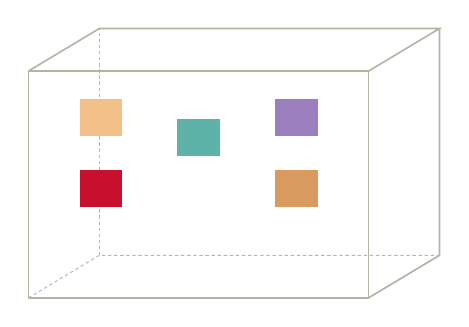
\begin{tikzpicture}
        \cubeShape{3.6}{0}{0}
      \end{tikzpicture}
    \end{column}
    \begin{column}{8.4cm}
      \eyebrow{Phase 0 / proposal sketch / \today}\par
      \vspace{14pt}
      {\displayfont\fontsize{34pt}{38pt}\selectfont\color{textPrimary}%
       Workforce Pell\\at SOU\par}
      \vspace{14pt}
      {\color{oil}\rule{2.6em}{0.7pt}}\par
      \vspace{14pt}
      {\rmfamily\itshape\fontsize{14pt}{18pt}\selectfont
       \color{textSecondary}A bioregional revenue strategy\\
       for the Rogue Valley.\par}
      \vspace{22pt}
      \monoLabel{daniel defreez / southern oregon university}
    \end{column}
  \end{columns}
\end{frame}
}

% ====================================================================
% 1.  The moment
% ====================================================================
\frametitleEyebrow{SOU / financial inflection}
\begin{frame}{We are looking for new revenue. One arrives in eight weeks.}
  \begin{columns}[T,onlytextwidth]
    \begin{column}{0.58\textwidth}
      \rmfamily\fontsize{11.5pt}{15.5pt}\selectfont
      \color{textPrimary}
      Southern Oregon University is drafting a downsizing
      proposal and has asked the public for revenue ideas that
      could supplement existing academic tracks.\par
      \vspace{8pt}
      On \textbf{July 20, 2026}, a new federal program takes
      effect that universities are uniquely positioned to
      deliver: \textbf{Workforce Pell}.\par
      \vspace{8pt}
      This deck proposes one new track:
      \textbf{SOU as the Rogue Valley's bioregional hub for
      applied learning} \textemdash{} short, employer-aligned,
      Pell-funded certificate programs that ladder into
      existing SOU degrees.\par
      \vspace{10pt}
      \color{textSecondary}\itshape\fontsize{10pt}{13.5pt}\selectfont
      A new revenue category. Federally backed. Anchored in
      regional demand. No tuition risk to the student.
    \end{column}
    \begin{column}{0.40\textwidth}
      \centering
      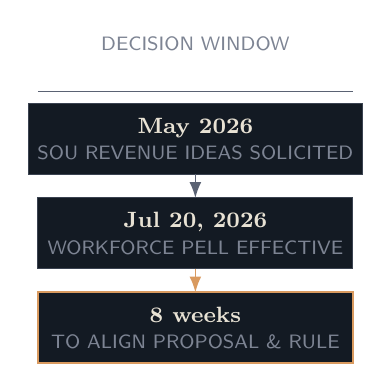
\begin{tikzpicture}[every node/.style={align=center,font=\scriptsize\sffamily,
                                             text=textPrimary}]
        \node[anchor=south,font=\scriptsize\sffamily,text=textMuted]
              at (0,2.7) {\eyebrow{decision window}};
        \draw[lineStrong,line width=0.6pt] (-2.0,2.3) -- (2.0,2.3);
        \node[draw=lineMid,line width=0.4pt,fill=bgRaised,
              minimum width=4.0cm,minimum height=0.9cm,
              text=textPrimary,font=\footnotesize\rmfamily]
              at (0,1.7) {\textbf{May 2026}\\\eyebrow{SOU revenue ideas solicited}};
        \node[draw=lineMid,line width=0.4pt,fill=bgRaised,
              minimum width=4.0cm,minimum height=0.9cm,
              text=textPrimary,font=\footnotesize\rmfamily]
              at (0,0.5) {\textbf{Jul 20, 2026}\\\eyebrow{Workforce Pell effective}};
        \node[draw=oil,line width=0.7pt,fill=bgRaised,
              minimum width=4.0cm,minimum height=0.9cm,
              text=textPrimary,font=\footnotesize\rmfamily]
              at (0,-0.7) {\textbf{8 weeks}\\\eyebrow{to align proposal \& rule}};
        \draw[-{Latex[length=2mm]},draw=lineStrong,line width=0.5pt]
              (0,1.25) -- (0,0.95);
        \draw[-{Latex[length=2mm]},draw=oil,line width=0.6pt]
              (0,0.05) -- (0,-0.25);
      \end{tikzpicture}
    \end{column}
  \end{columns}
\end{frame}

% ====================================================================
% 2.  What is Workforce Pell?
% ====================================================================
\frametitleEyebrow{Federal / Workforce Pell Grant}
\begin{frame}{A new Pell category for short, high-quality, employment-aligned programs}
  \begin{columns}[T,onlytextwidth]
    \begin{column}{0.52\textwidth}
      \rmfamily\fontsize{10pt}{13pt}\selectfont
      \color{textPrimary}
      \eyebrow{program shape}
      \vspace{2pt}
      \begin{itemize}\itemsep1pt
        \item \textbf{8\textendash15 weeks} of instructional time
        \item \textbf{150\textendash599 clock hours}, or equivalent credit
        \item No correspondence, remedial, or study-abroad
        \item Must be offered by an \textbf{accredited institution}
      \end{itemize}
      \vspace{8pt}
      \eyebrow{three annual federal thresholds}
      \vspace{2pt}
      \begin{itemize}\itemsep1pt
        \item \textbf{70\%} of participants complete within 150\% of normal time
        \item \textbf{70\%} of completers employed in the 2nd quarter after exit
        \item Tuition + fees $\leq$ median completer earnings $-$
              150\% of the federal poverty line\\
              {\color{textMuted}\scriptsize(2026: 150\% of poverty $\approx$ \$23{,}475 for an individual)}
      \end{itemize}
    \end{column}
    \begin{column}{0.46\textwidth}
      \rmfamily\fontsize{10pt}{13pt}\selectfont
      \color{textPrimary}
      \eyebrow{approval path}
      \vspace{2pt}
      \begin{itemize}\itemsep1pt
        \item \textbf{Governor} approves first, after consulting the
              State Workforce \& Talent Development Board
        \item \textbf{Secretary of Education} approves second
        \item Re-approval tied to institution's PPA expiration
      \end{itemize}
      \vspace{8pt}
      \eyebrow{notable provisions for universities}
      \vspace{2pt}
      \begin{itemize}\itemsep1pt
        \item \textbf{Bachelor's-degree holders are eligible} \textemdash{}
              rare in Pell
        \item \textbf{Employers may deliver up to 25\%} of instruction\\
              (\textbf{49\%} for Registered Apprenticeship Programs)
        \item Programs must award academic credit toward an
              existing certificate or degree
      \end{itemize}
      \vspace{8pt}
      \monoLabel{Source: ED Final Rule Fact Sheet, May 18, 2026 \textbullet{} Federal Register, May 19, 2026.}
    \end{column}
  \end{columns}
\end{frame}

% ====================================================================
% 3.  Why universities
% ====================================================================
\frametitleEyebrow{Position / why higher-ed wins this}
\begin{frame}{Workforce Pell was written for institutions like SOU}
  \centering
  \rmfamily\fontsize{9.5pt}{12.5pt}\selectfont
  \color{textPrimary}
  \renewcommand{\arraystretch}{1.32}
  \begin{tabular}{@{}p{4.6cm}p{8.8cm}@{}}
    \toprule
    \eyebrow{federal requirement} & \eyebrow{what it means for SOU}\\
    \midrule
    Accredited institution; 5 clean years
      & For-profit short-course providers are excluded by design. SOU clears.\\
    \addlinespace[2pt]
    Stackable / credit-bearing credential
      & The program must award academic credit toward an existing certificate or degree. \textbf{Universities already own the ladder.}\\
    \addlinespace[2pt]
    Up to 25\% employer-delivered (49\% in RAP)
      & SOU partners with regional employers and apprenticeship sponsors; the university orchestrates while industry contributes hours.\\
    \addlinespace[2pt]
    Governor + WTDB alignment to regional demand
      & SOU already engages HECC and the Rogue Workforce Partnership through CTE and WIOA channels. The relationships exist.\\
    \addlinespace[2pt]
    Three annual outcome tests
      & The metrics (completion, employment, value-added earnings) are precisely what a university outcomes office can defend.\\
    \bottomrule
  \end{tabular}
  \vspace{10pt}\par
  {\itshape\color{textSecondary}\fontsize{10pt}{13.5pt}\selectfont
   For-profit short-course providers cannot meet most of this.
   Community colleges share the lane, but lack the bachelor's-ladder
   pathway that the rule explicitly rewards.}
\end{frame}

% ====================================================================
% 4.  Why SOU specifically
% ====================================================================
\frametitleEyebrow{Position / bioregional anchor}
\begin{frame}{SOU as the Rogue Valley's bioregional hub for applied learning}
  \begin{columns}[T,onlytextwidth]
    \begin{column}{0.50\textwidth}
      \rmfamily\fontsize{10.5pt}{14pt}\selectfont
      \color{textPrimary}
      \eyebrow{bioregional positioning}
      \vspace{4pt}
      \begin{itemize}\itemsep2pt
        \item Anchor institution for Jackson and Josephine counties.
        \item Existing capacity in healthcare, education,
              business, sustainability, and outdoor sciences.
        \item Faculty and facilities already cleared for accredited
              credentialing.
        \item Sits next to the Rogue Workforce Partnership and
              Business Oregon's southern Oregon office.
      \end{itemize}
      \vspace{8pt}
      \color{textSecondary}\itshape\fontsize{10pt}{13.5pt}\selectfont
      A Workforce Pell track is not a pivot \textemdash{} it is a
      repackaging of existing SOU strengths into shorter,
      employer-aligned credentials that ladder back into degrees.
    \end{column}
    \begin{column}{0.48\textwidth}
      \centering
      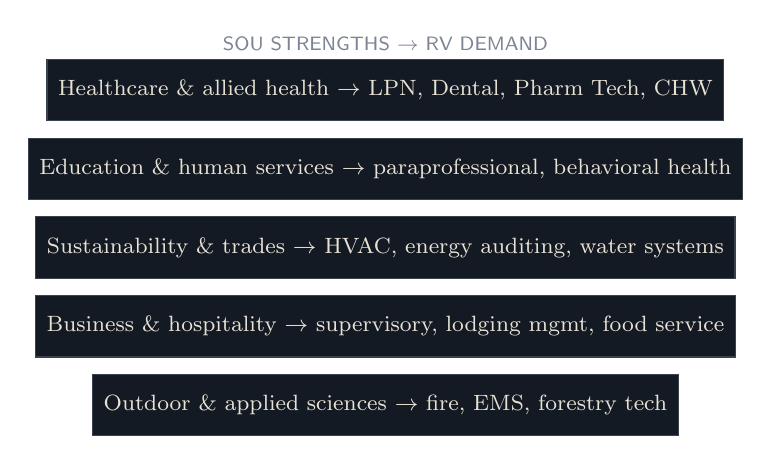
\begin{tikzpicture}[
          every node/.style={font=\scriptsize\sffamily,
                             text=textPrimary,align=center},
          band/.style={draw=lineMid,line width=0.4pt,fill=bgRaised,
                       minimum width=5.6cm,minimum height=0.78cm,
                       text=textPrimary,inner sep=4pt,
                       font=\footnotesize\rmfamily},
        ]
        \node[anchor=north,text=textMuted] at (0,3.4) {\eyebrow{SOU strengths $\rightarrow$ RV demand}};
        \node[band] (b1) at (0, 2.6) {Healthcare \& allied health $\rightarrow$ LPN, Dental, Pharm Tech, CHW};
        \node[band] (b2) at (0, 1.6) {Education \& human services $\rightarrow$ paraprofessional, behavioral health};
        \node[band] (b3) at (0, 0.6) {Sustainability \& trades $\rightarrow$ HVAC, energy auditing, water systems};
        \node[band] (b4) at (0,-0.4) {Business \& hospitality $\rightarrow$ supervisory, lodging mgmt, food service};
        \node[band] (b5) at (0,-1.4) {Outdoor \& applied sciences $\rightarrow$ fire, EMS, forestry tech};
      \end{tikzpicture}
    \end{column}
  \end{columns}
\end{frame}

% ====================================================================
% 5.  RV occupation demand
% ====================================================================
\frametitleEyebrow{Evidence / Rogue Valley demand}
\begin{frame}{Six RV occupations that fit Workforce Pell today}
  \centering
  \rmfamily\fontsize{9.4pt}{12pt}\selectfont
  \color{textPrimary}
  \renewcommand{\arraystretch}{1.22}
  \begin{tabular}{@{}p{4.8cm}rrr@{}}
    \toprule
    \eyebrow{occupation (SOC)}
      & \eyebrow{RV 10-yr openings}
      & \eyebrow{2025 median wage}
      & \eyebrow{value-added cap}\\
    \midrule
    Licensed Practical / Vocational Nurses
      & 325 & \$79{,}414 & \$55{,}939\\
    \addlinespace[2pt]
    Dental Assistants
      & 572 & \$56{,}514 & \$33{,}039\\
    \addlinespace[2pt]
    Pharmacy Technicians
      & 355 & \$54{,}746 & \$31{,}271\\
    \addlinespace[2pt]
    Surgical Technologists
      &  81 & \$76{,}877 & \$53{,}402\\
    \addlinespace[2pt]
    HVAC \& Refrigeration Mechanics
      & 231 & \$61{,}048 & \$37{,}573\\
    \addlinespace[2pt]
    Community Health Workers
      &  86 & \$58{,}490 & \$35{,}015\\
    \bottomrule
  \end{tabular}
  \vspace{10pt}\par
  {\itshape\color{textSecondary}\fontsize{10pt}{13.5pt}\selectfont
   ``Value-added cap'' = the federal tuition + fees ceiling per student\\
   (median wage $-$ \$23{,}475). Every line above is a defensible
   revenue envelope.}\par
  \vspace{6pt}
  \monoLabel{Source: Oregon Employment Department, Rogue Valley High-Wage, High-Demand, High-Skill Occupations 2024\textendash 2034.}
\end{frame}

% ====================================================================
% 6.  One cell populated (RV WIOA outcomes)
% ====================================================================
\frametitleEyebrow{Evidence / RV workforce outcomes that already exist}
\begin{frame}{The Rogue Valley already outperforms statewide on outcomes}
  \centering
  \rmfamily\fontsize{9.4pt}{11.6pt}\selectfont
  \color{textPrimary}
  \renewcommand{\arraystretch}{1.22}
  \begin{tabular}{@{}p{6.2cm}rr@{}}
    \toprule
    \eyebrow{WIOA outcome (2023, all programs)}
      & \eyebrow{rogue valley}
      & \eyebrow{statewide}\\
    \midrule
    Total WIOA participants
      & 1{,}230 & 8{,}134\\
    \addlinespace[2pt]
    Measurable Skill Gain rate
      & 60\% & 67\%\\
    \addlinespace[2pt]
    Credential attainment (exiters)
      & \textbf{64\%} & 66\%\\
    \addlinespace[2pt]
    Employment, 2 quarters after exit
      & \textbf{71\%} & 65\%\\
    \addlinespace[2pt]
    Employment, 4 quarters after exit
      & \textbf{66\%} & 63\%\\
    \addlinespace[2pt]
    Median earnings, 2 quarters after exit
      & \$8{,}500 & \$9{,}000\\
    \bottomrule
  \end{tabular}
  \vspace{10pt}\par
  {\itshape\color{textSecondary}\fontsize{10pt}{13.5pt}\selectfont
   The Rogue Valley clears the 70\% employment threshold today.
   The 70\% completion threshold is the bar SOU's track would
   be designed to meet.}\par
  \vspace{6pt}
  \monoLabel{Source: HECC WIOA Title I Workforce Data Dashboard (2023). Extract: SOURVWF/Statewide/oregon-wioa-dashboard/.}
\end{frame}

% ====================================================================
% 7.  Why HECC's dashboard isn't enough
% ====================================================================
\frametitleEyebrow{Adjacent / what current data can and cannot do}
\begin{frame}{HECC's WIOA dashboard answers part of this, not most}
  \begin{columns}[T,onlytextwidth]
    \begin{column}{0.48\textwidth}
      \rmfamily\fontsize{10pt}{13pt}\selectfont
      \color{textPrimary}
      \eyebrow{what HECC publishes today}
      \vspace{4pt}
      \begin{itemize}\itemsep1pt
        \item WIOA Title I participants \& demographics
        \item Measurable Skill Gains
        \item Credential attainment by exit year
        \item Employment 2Q \& 4Q after exit
        \item Median earnings 2Q \& 4Q after exit
        \item Filter by local workforce board, program year
      \end{itemize}
    \end{column}
    \begin{column}{0.48\textwidth}
      \rmfamily\fontsize{10pt}{13pt}\selectfont
      \color{textPrimary}
      \eyebrow{what HECC does \textit{not} publish}
      \vspace{4pt}
      \begin{itemize}\itemsep1pt
        \item Non-WIOA training (most CTE; Pell-eligible workforce)
        \item Employer demand (no QCEW or postings join)
        \item Per-program ROI (cannot rank programs)
        \item Wages by SOC (only by exiter demographic)
        \item Sub-board geography (no Jackson / Josephine split)
        \item Real-time intake (annual; lags ${\sim}$2 years)
        \item Coverage diagnostic (no signal on thin evidence)
      \end{itemize}
    \end{column}
  \end{columns}
  \vspace{8pt}
  \begin{center}
    \itshape\color{textSecondary}\fontsize{10.5pt}{13.5pt}\selectfont
    The right-hand list is exactly what Workforce Pell will ask
    the Governor to attest. We need a data layer that fills it
    \textemdash{} \textbf{Ashland Intelligence}, sketched on
    the next slide.
  \end{center}
\end{frame}

% ====================================================================
% 8.  Ashland Intelligence engine (brief)
% ====================================================================
\frametitleEyebrow{Engine / the data layer that makes filings defensible}
\begin{frame}{Ashland Intelligence: the data engine, not the headline}
  \begin{columns}[T,onlytextwidth]
    \begin{column}{0.52\textwidth}
      \rmfamily\fontsize{10.5pt}{14pt}\selectfont
      \color{textPrimary}
      A regional intelligence layer joining employer demand,
      institutional capacity, and federal predicates into one
      auditable evidence base for Workforce Pell filings.\par
      \vspace{8pt}
      \begin{itemize}\itemsep2pt
        \item Composes sources \textemdash{} HECC, OED, RWP,
              SOREDI, Business Oregon, FAFSA \textemdash{} on
              one schema.
        \item Powers the \textbf{Annotated Ledger}, SOU's
              budget-data dashboard, with regional labor signal.
        \item Published quarterly; every output cites its source.
      \end{itemize}
      \vspace{6pt}
      \color{textSecondary}\itshape\fontsize{10pt}{13pt}\selectfont
      Ashland Intelligence is the operational substrate. Workforce
      Pell at SOU is what it enables first.
    \end{column}
    \begin{column}{0.46\textwidth}
      \centering
      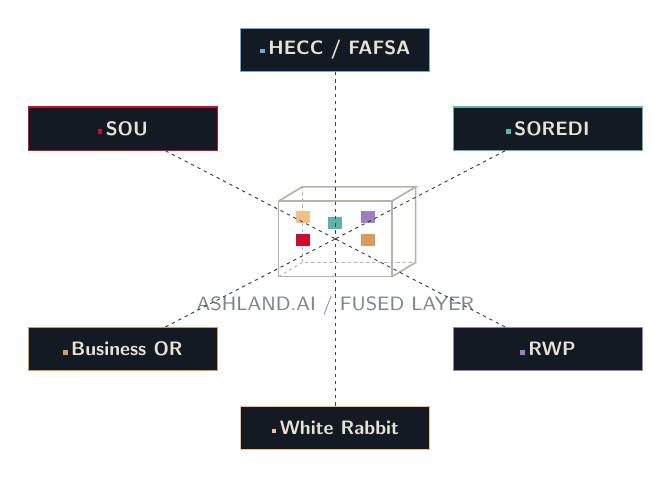
\begin{tikzpicture}[
          every node/.style={font=\footnotesize\sffamily,
                             text=textPrimary,align=center},
          seat/.style={draw=lineMid,line width=0.4pt,fill=bgRaised,
                       text=textPrimary,
                       minimum height=0.55cm,minimum width=2.4cm,
                       inner sep=4pt,
                       font=\scriptsize\sffamily},
        ]
        \cubeShape{1.2}{0}{0}
        \node[font=\scriptsize\sffamily,text=textMuted,
              anchor=north] at (0,-0.6)
              {\eyebrow{ashland.ai / fused layer}};
        \node[seat,draw=cSou]    (s1) at (-2.7, 1.4) {\pdot{cSou}\,\textbf{SOU}};
        \node[seat,draw=cSoredi] (s2) at ( 2.7, 1.4) {\pdot{cSoredi}\,\textbf{SOREDI}};
        \node[seat,draw=cBiz]    (s3) at (-2.7,-1.4) {\pdot{cBiz}\,\textbf{Business OR}};
        \node[seat,draw=cRwp]    (s4) at ( 2.7,-1.4) {\pdot{cRwp}\,\textbf{RWP}};
        \node[seat,draw=cPell]   (s5) at (0,  2.4)   {\pdot{cPell}\,\textbf{HECC / FAFSA}};
        \node[seat,draw=cWr]     (s6) at (0, -2.4)   {\pdot{cWr}\,\textbf{White Rabbit}};
        \foreach \s in {s1,s2,s3,s4,s5,s6}
          \draw[lineMid,line width=0.35pt,dashed,
                dash pattern=on 1.2pt off 1.4pt]
                (\s) -- (0,0);
      \end{tikzpicture}
    \end{column}
  \end{columns}
\end{frame}

% ====================================================================
% 9.  Anatomy of a SOU Workforce Pell program
% ====================================================================
\frametitleEyebrow{Operating model / program anatomy}
\begin{frame}{Anatomy of a SOU Workforce Pell program}
  \vspace{0.1cm}
  \begin{columns}[T,onlytextwidth,totalwidth=\textwidth]
    \begin{column}{0.25\textwidth}\centering
      \schemCard{curriculum}{%
        8\textendash15 weeks.\\
        150\textendash599 clock hours.\\
        Employer-validated competencies.\\
        Industry-recognized assessments.\\[6pt]
        {\itshape\color{textMuted}built once, run repeatedly.}%
      }{cPell}
    \end{column}
    \begin{column}{0.25\textwidth}\centering
      \schemCard{delivery}{%
        SOU faculty + up to 25\%\\
        employer-delivered hours.\\
        (49\% via Registered\\
        Apprenticeship.)\\[6pt]
        {\itshape\color{textMuted}distributed teaching,\\
         university orchestration.}%
      }{cSou}
    \end{column}
    \begin{column}{0.25\textwidth}\centering
      \schemCard{credential}{%
        Stackable to existing\\
        SOU certificate, AA,\\
        or BA pathway.\\
        Counts as academic credit.\\[6pt]
        {\itshape\color{textMuted}an entry, not a dead end.}%
      }{cRwp}
    \end{column}
    \begin{column}{0.25\textwidth}\centering
      \schemCard{outcomes}{%
        $\geq$\,70\% completion.\\
        $\geq$\,70\% employed 2Q after.\\
        Tuition $\leq$ value-added\\
        earnings cap.\\[6pt]
        {\itshape\color{textMuted}defensible to the\\
         Governor and Secretary.}%
      }{oil}
    \end{column}
  \end{columns}
  \vspace{12pt}\par
  \centering
  {\itshape\color{textSecondary}\fontsize{10pt}{13pt}\selectfont
   Each program approved first by the Governor in consultation
   with the State Workforce \& Talent Development Board,
   then by the U.S. Secretary of Education.}
\end{frame}

% ====================================================================
% 10. Revenue model
% ====================================================================
\frametitleEyebrow{Numbers / what this looks like as a revenue line}
\begin{frame}{Each completer is a defensible new revenue line for SOU}
  \begin{columns}[T,onlytextwidth]
    \begin{column}{0.50\textwidth}
      \rmfamily\fontsize{10pt}{13.5pt}\selectfont
      \color{textPrimary}
      \eyebrow{the per-student revenue envelope}
      \vspace{4pt}
      \begin{itemize}\itemsep2pt
        \item Federal cap on tuition + fees =\\
              median completer earnings $-$ \$23{,}475
        \item For a \$60{,}000-median-earnings program:\\
              cap $\approx$ \textbf{\$36{,}525 per student}
        \item Even a conservative \$5{,}000\textendash\$10{,}000 tuition fits comfortably below the cap.
        \item Pell pays. Student carries no debt; SOU is paid up-front.
      \end{itemize}
      \vspace{8pt}
      \eyebrow{worked example}
      \vspace{4pt}
      \rmfamily\fontsize{10pt}{13pt}\selectfont
      3 pilot programs $\times$ 30 completers $\times$ \$8{,}000
      net tuition $=$ \textbf{\$720{,}000 annual recurring}.\\
      Scale to 6 programs $\times$ 50 completers $=$
      \textbf{\$2.4M annual recurring}, modest capex,
      faculty shareable with degree tracks.
    \end{column}
    \begin{column}{0.46\textwidth}
      \centering
      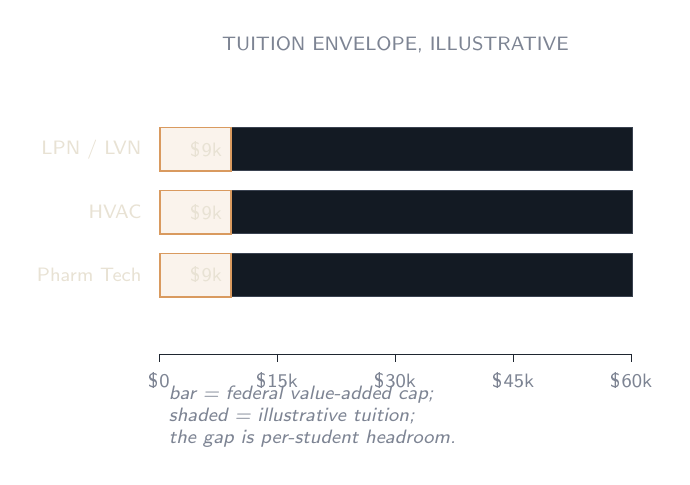
\begin{tikzpicture}[
          every node/.style={font=\scriptsize\sffamily,
                             text=textPrimary,align=center},
          bar/.style={draw=lineMid,line width=0.4pt,fill=bgRaised},
          accent/.style={draw=oil,line width=0.6pt,fill=oil!12},
        ]
        \node[anchor=south,text=textMuted] at (3,3.7)
              {\eyebrow{tuition envelope, illustrative}};
        % horizontal scale
        \draw[lineSoft,line width=0.3pt] (0,0) -- (6,0);
        \foreach \x/\lab in {0/0,1.5/15k,3/30k,4.5/45k,6/60k} {
          \draw[lineSoft,line width=0.3pt] (\x,0) -- (\x,-0.1);
          \node[anchor=north,font=\scriptsize\sffamily,text=textMuted]
                at (\x,-0.12) {\$\lab};
        }
        % bars (each = a program)
        \node[bar,minimum width=6cm,minimum height=0.55cm,anchor=west]
              (b1) at (0,1.0) {};
        \node[anchor=east,font=\scriptsize\sffamily,text=textPrimary]
              at (-0.1,1.0) {Pharm Tech};
        \node[accent,minimum width=0.9cm,minimum height=0.55cm,anchor=west]
              at (0,1.0) {};
        \node[font=\scriptsize\sffamily,text=textPrimary] at (0.6,1.0) {\$9k};

        \node[bar,minimum width=6cm,minimum height=0.55cm,anchor=west]
              (b2) at (0,1.8) {};
        \node[anchor=east,font=\scriptsize\sffamily,text=textPrimary]
              at (-0.1,1.8) {HVAC};
        \node[accent,minimum width=0.9cm,minimum height=0.55cm,anchor=west]
              at (0,1.8) {};
        \node[font=\scriptsize\sffamily,text=textPrimary] at (0.6,1.8) {\$9k};

        \node[bar,minimum width=6cm,minimum height=0.55cm,anchor=west]
              (b3) at (0,2.6) {};
        \node[anchor=east,font=\scriptsize\sffamily,text=textPrimary]
              at (-0.1,2.6) {LPN / LVN};
        \node[accent,minimum width=0.9cm,minimum height=0.55cm,anchor=west]
              at (0,2.6) {};
        \node[font=\scriptsize\sffamily,text=textPrimary] at (0.6,2.6) {\$9k};
        % annotation
        \node[anchor=west,font=\scriptsize\sffamily,text=textMuted,align=left]
              at (0,-0.8)
              {\textit{bar = federal value-added cap;}\\\textit{shaded = illustrative tuition;}\\\textit{the gap is per-student headroom.}};
      \end{tikzpicture}
    \end{column}
  \end{columns}
\end{frame}

% ====================================================================
% 11. Twelve months
% ====================================================================
\frametitleEyebrow{Cadence / twelve months}
\begin{frame}{Twelve months, five phases}
  \vspace{0.4cm}
  \centering
  \begin{tikzpicture}[
      every node/.style={font=\scriptsize\sffamily,
                         text=textPrimary,align=center},
      phase/.style={draw=lineMid,line width=0.4pt,fill=bgRaised,
                    inner sep=6pt,
                    minimum width=2.45cm,minimum height=1.95cm,align=center},
      arr/.style={-{Latex[length=1.8mm,width=1.4mm]},
                  draw=oil,line width=0.5pt},
    ]
    \node[phase] (p0)  at (-5.4,0)
      {{\sffamily\scriptsize\color{textMuted}PHASE 0}\\[2pt]
       \textbf{May 2026}\\[2pt]
       {\itshape\color{textMuted}scope 3 pilot\\programs}};
    \node[phase] (p1a) at (-2.7,0)
      {{\sffamily\scriptsize\color{textMuted}PHASE 1A}\\[2pt]
       \textbf{Jun--Aug 2026}\\[2pt]
       {\itshape\color{textMuted}Governor\\\& Secretary\\approval}};
    \node[phase] (p1b) at ( 0.0,0)
      {{\sffamily\scriptsize\color{textMuted}PHASE 1B}\\[2pt]
       \textbf{Sep--Nov 2026}\\[2pt]
       {\itshape\color{textMuted}first cohort\\enrolled}};
    \node[phase] (p1c) at ( 2.7,0)
      {{\sffamily\scriptsize\color{textMuted}PHASE 1C}\\[2pt]
       \textbf{Dec--Feb 2027}\\[2pt]
       {\itshape\color{textMuted}outcomes\\measurement\\begins}};
    \node[phase] (p2)  at ( 5.4,0)
      {{\sffamily\scriptsize\color{textMuted}PHASE 2}\\[2pt]
       \textbf{Mar--May 2027}\\[2pt]
       {\itshape\color{textMuted}first completers,\\first revenue}};
    \draw[arr] (p0)  -- (p1a);
    \draw[arr] (p1a) -- (p1b);
    \draw[arr] (p1b) -- (p1c);
    \draw[arr] (p1c) -- (p2);
    \node[anchor=north,text=textMuted,
          font=\scriptsize\itshape\rmfamily]
          at (0,-1.6)
          {Aligned to the first sustained Workforce Pell cohort cycles
           after the July 20, 2026 effective date.};
  \end{tikzpicture}
\end{frame}

% ====================================================================
% 12. Three asks
% ====================================================================
\frametitleEyebrow{Closing / three asks}
\begin{frame}{Three asks}
  \centering
  \rmfamily\fontsize{9pt}{12.2pt}\selectfont
  \color{textPrimary}
  \renewcommand{\arraystretch}{1.34}
  \begin{tabular}{@{}p{3.6cm}p{10.0cm}@{}}
    \toprule
    \eyebrow{audience} & \eyebrow{the ask}\\
    \midrule
    \pdot{cSou}\,\textbf{SOU officials}
      & Include a \textbf{Workforce Pell track} in the revenue-diversification proposal. Designate a project lead within 30 days. Pick three pilot programs from the RV demand list (e.g.\ LPN, Dental Assistant, HVAC).\\
    \addlinespace[2pt]
    \pdot{cPell}\,\textbf{HECC + WTDB}
      & Use the existing \textbf{Oregon CTE Skill Cluster framework} as the alignment basis for Governor approval criteria. Use the \textbf{Rogue Workforce Partnership 2024\textendash 2028 Local Plan} as the regional demand evidence base. Do not re-invent. The standards exist.\\
    \addlinespace[2pt]
    \pdot{cRwp}\,\textbf{Community \& RV partners}
      & Provide employer intent letters and internship slots for the first three programs. Advocate locally and at HECC. Help SOU run the data engine that makes the filing defensible.\\
    \bottomrule
  \end{tabular}
  \vspace{14pt}\par
  {\itshape\color{textSecondary}\fontsize{10.5pt}{14pt}\selectfont
   Eight weeks to the federal effective date. The fastest path is\\
   to bring SOU's existing strengths into the rule's open door.}\par
  \vspace{10pt}
  {\sffamily\fontsize{8pt}{10pt}\selectfont\color{textMuted}
   The Rogue Valley first. Statewide in 2027.}
\end{frame}

\end{document}
